\begin{rightcolumn}

\subsubsection{Valor Potencial con mejoras internas.}

Se utilizó una metodología de valuación de negocios basada en el punto número 3 del pentágono de explotación de oportunidades, conocido como \textit{valor actual interno}. Lo anterior  implica realizar el análisis de valor del activo intangible en las condiciones que opera al día de hoy; esto es, sin realizar ninguna explotación de oportunidades en los factores internos y externos. (\autoref{fig:hexagono}) \\

``\textcolor{secundario}{Valor potencial con mejoras internas}.- Es el valor que adquiere la unidad econ\'omica valuada una vez que se realiz\'o la identificaci\'on y explotaci\'on de los factores internos. Para lo cual se corrigen deficiencias, se mejoran y optimizan procesos y se explotan nuevas oportunidades estrat\'egicas, obteni\'endose as\'i un mayor valor de la unidad econ\'omica''\\

\end{rightcolumn}
\begin{leftcolumn}

\begin{figure}[H]
\centering
\caption{Pent\'agono de Explotaci\'on de oportunidades\label{fig:hexagono}}
\includegraphics[width=5cm]{\rutaImagenes/pentagono}\\
Fuente:Valuation. Copeland Tom, Koller Tim y Murrin Jack.\\

John Wiley \& Sons. 2000.
\end{figure}

\end{leftcolumn}

